% ===========================================================================
% Methology
% File: sections/03_methodology.tex
% Built sub-section by sub-section
% ===========================================================================

\section{Methodology}
\label{sec:method}

% ---------------------------------------------------------------------------

% ---------------------------------------------------------------------------
\subsection{Study Sites and Climate Data}
\label{sec:sites}
% ---------------------------------------------------------------------------

\hspace{1cm}Four sites were selected to span four distinct K\"{o}ppen--Geiger
climate subtypes across a latitudinal range of \SI{12}{\degree}N to
\SI{48}{\degree}N (Table~\ref{tab:sites}, Figure~\ref{fig:sitemap}).
The selection criterion was maximum climate diversity within the semi-arid
and adjacent temperate zones that represent the primary deployment contexts
for agrivoltaic systems: two hot and cold semi-arid sites (Almer\'{i}a
BSh and Konya BSk), one tropical semi-arid site (Ouagadougou BSh), and
one oceanic temperate site (Freiburg Cfb) included as a northern European
reference.

\begin{figure}[H]
\centering
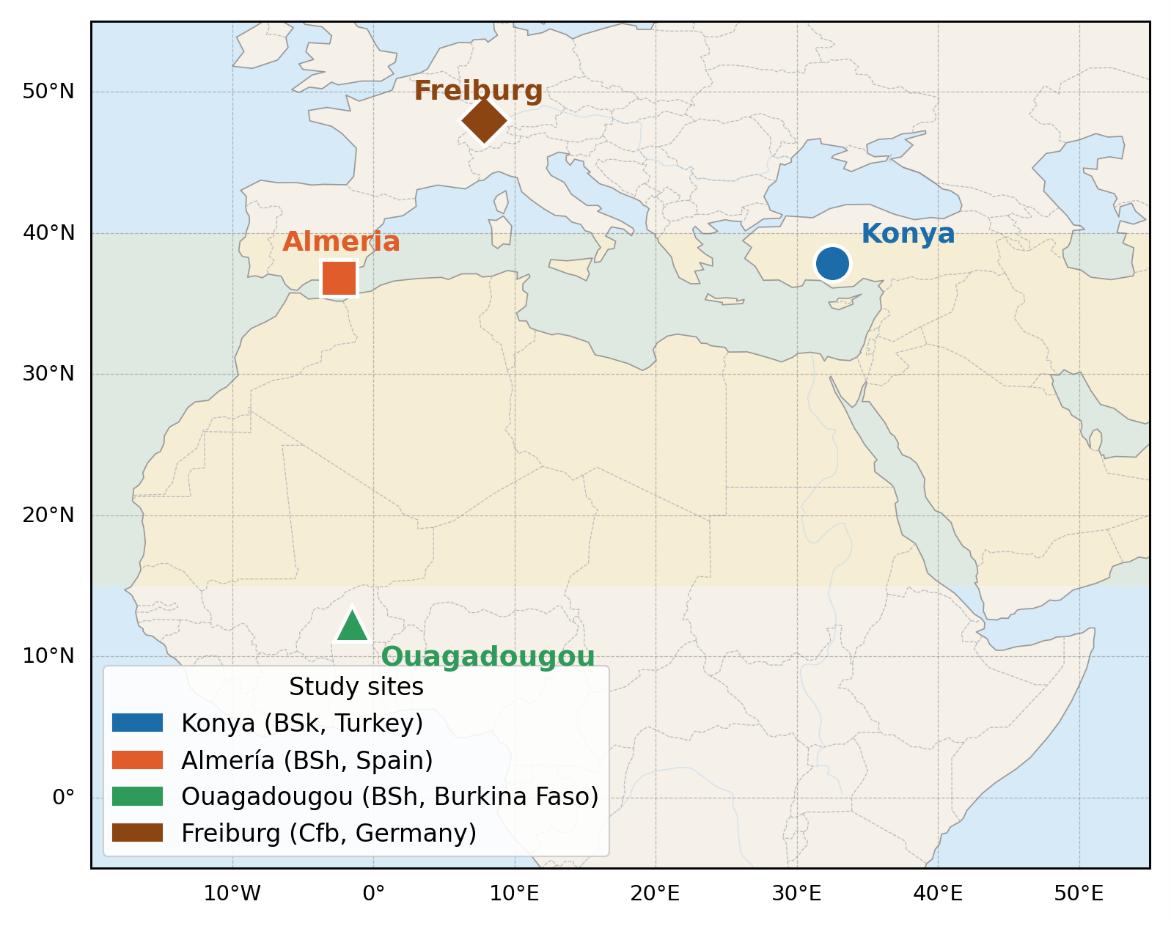
\includegraphics[width=\textwidth]{figures/fig01_site_map.png}
\caption{Location map of the four study sites overlaid on the
K\"{o}ppen--Geiger climate classification. Semi-arid zones (BS)
are shaded in light yellow; the oceanic temperate zone (Cfb) in
light blue.}
\label{fig:sitemap}
\end{figure}

Hourly climate data were obtained from the PVGIS-SARAH3 Typical
Meteorological Year (TMY) database of the European Commission Joint
Research Centre~\citep{pvgis, huld2012}. The SARAH3 satellite product
provides direct normal irradiance (DNI) and diffuse horizontal irradiance
(DHI) as independent retrievals, without decomposition from global
horizontal irradiance (GHI). This avoids the systematic decomposition
errors of up to $\pm$8\% reported for empirical decomposition models
under broken cloud conditions~\citep{urraca2017}. The mean bias error
of PVGIS-SARAH3 GHI estimates is below $\pm$5\% for monthly averages
at all four study sites~\citep{huld2012}. The TMY file format provides
ten meteorological variables at hourly resolution (8760 rows per site):
air temperature T$_{2m}$ (\si{\celsius}), relative humidity RH (\%),
GHI, DNI, DHI (W\,m$^{-2}$), downwelling infrared irradiance IR(h)
(W\,m$^{-2}$), 10-m wind speed WS$_{10m}$ (m\,s$^{-1}$), wind
direction WD$_{10m}$ (°), and surface pressure SP (Pa).

\begin{table}[H]
\caption{Geographical and climatic characteristics of the four study
sites (PVGIS-SARAH3 TMY data).}
\label{tab:sites}
\centering
\begin{tabular}{p{4cm}cccc}
\toprule
\textbf{Parameter} & \textbf{Konya} & \textbf{Almer\'{i}a}
    & \textbf{Ouagadougou} & \textbf{Freiburg} \\
\midrule
Latitude            & 37.87°N & 36.83°N & 12.37°N & 47.99°N \\
Longitude           & 32.49°E & 2.46°W  & 1.52°W  & 7.85°E  \\
Elevation (m a.s.l.)& 1\,016  & 20      & 303     & 278     \\
K\"{o}ppen class    & BSk     & BSh     & BSh     & Cfb     \\
Annual GHI (kWh\,m$^{-2}$) & 1\,650 & 1\,850 & 2\,050 & $\sim$1\,150 \\
Mean annual T (\si{\celsius}) & 11.5 & 18.5 & 28.5 & $\sim$11.4 \\
Summer T$_{\max}$ (\si{\celsius}) & 38 & 35 & 41 & $\sim$35 \\
Winter T$_{\min}$ (\si{\celsius}) & $-$10 & $+$5 & $+$15 & $\sim{-12}$ \\
Annual ET$_0$ (mm)  & 1\,200  & 1\,350  & 1\,800  & $\sim$900 \\
Annual precip. (mm) & 320     & 200     & 800     & $\sim$800 \\
\bottomrule
\end{tabular}
\end{table}

\begin{figure}[H]
\centering

\includegraphics[width=\textwidth]{figures/fig02_climate_profiles.png}
\caption{Monthly climate profiles for the four study sites from
PVGIS-SARAH3 TMY data. Upper row: monthly GHI (kWh\,m$^{-2}$)
with annual total annotated; lower row: mean monthly air temperature
(\si{\celsius}). Shaded bands indicate the tomato growing season
at each site.}
\label{fig:climateprofiles}
\end{figure}

The four sites span a mean annual temperature range of
11.4--28.5\,\si{\celsius}, a GHI range of 1\,150--2\,050\,kWh\,m$^{-2}$,
and growing seasons of 122--189 days. This diversity ensures that the
model is tested across the full range of Arrhenius BMP suppression
(from negligible at Ouagadougou to severe at Freiburg in January)
and PAR saturation regimes (from frequent saturation at Ouagadougou
to rare saturation at Freiburg), providing the basis for the
multi-climate findings reported in Section~\ref{sec:results}.

% ---------------------------------------------------------------------------
\subsection{Crop Parameters and Growing Seasons}
\label{sec:crop}
% ---------------------------------------------------------------------------

\hspace{1cm}Tomato (\textit{Solanum lycopersicum}) was selected as the
reference crop for all four sites on the basis of three criteria: it is
cultivated commercially in all four study regions, its PAR saturation
point (\SI{174}{W\,m^{-2}}) is well-documented and places it in the
high-irradiance sensitivity range where APV shading effects are most
pronounced, and its residue-to-fruit ratio and BMP are among the
best-characterised in the agrivoltaic and AD
literatures~\citep{mohammedi2023, lallement2023, feng2013}.

Site-specific planting and harvest dates follow local agricultural
calendars (Table~\ref{tab:crop}). The three semi-arid sites use a fresh
fruit yield of \SI{60}{t\,ha^{-1}}, consistent with irrigated greenhouse
and open-field production in Mediterranean and tropical semi-arid
contexts~\citep{mohammedi2023}. Freiburg uses \SI{30}{t\,ha^{-1}}
following German open-field production statistics~\citep{dlg2023}.

\begin{table}[H]
\caption{Site-specific agronomic, economic, and environmental parameters.
Grid emission factors (EF) from \citet{iea2025} and Umweltbundesamt (2023).
Carbon prices from EU ETS (2024) for Almer\'{i}a and Freiburg;
voluntary market rates for Konya and Ouagadougou.}
\label{tab:crop}
\centering
\begin{tabular}{lcccc}
\toprule
\textbf{Parameter} & \textbf{Konya} & \textbf{Almer\'{i}a}
    & \textbf{Ouagadougou} & \textbf{Freiburg} \\
\midrule
Planting date           & 25 Apr  & 1 Mar   & 1 Jul   & 1 May   \\
Harvest date            & 30 Oct  & 30 Jun  & 30 Oct  & 15 Oct  \\
Season length (days)    & 189     & 122     & 122     & 167     \\
Fruit yield (t\,ha$^{-1}$) & 60  & 60      & 60      & 30      \\
Season ET$_0$ (mm)      & 650     & 480     & 620     & $\sim$350 \\
Residue ratio $R_{\text{res}}$ & \multicolumn{4}{c}{0.80~\citep{mohammedi2023}} \\
Dry matter $DM$ (tomato residues) & \multicolumn{4}{c}{0.06~\citep{mohammedi2023}} \\
VS fraction $VS_f$      & \multicolumn{4}{c}{0.85~\citep{lallement2023}} \\
Manure input (t\,ha$^{-1}$\,yr$^{-1}$) & \multicolumn{4}{c}{10.0} \\
Manure $DM_m$           & \multicolumn{4}{c}{0.20~\citep{pilarski2025}} \\
Manure $VS_m$           & \multicolumn{4}{c}{0.80~\citep{pilarski2025}} \\
\midrule
Tomato price (\$\,t$^{-1}$) & 300 & 400  & 250     & 350     \\
Electricity price (\$\,kWh$^{-1}$) & 0.06 & 0.09 & 0.12 & 0.09 \\
Discount rate (\%)      & 8       & 6       & 10      & 5       \\
Grid EF (tCO$_2$\,MWh$^{-1}$) & 0.438 & 0.167 & 0.632 & 0.380 \\
Carbon price (\$\,tCO$_2^{-1}$) & 15  & 65    & 12      & 65      \\
\bottomrule
\end{tabular}
\end{table}

The feedstock to the anaerobic digester combines tomato crop residues
and cattle manure as a co-substrate. Manure co-digestion at a VS ratio
of approximately 1:2 (residues:manure) improves buffer capacity,
microbial diversity, and BMP by 12--18\% compared to mono-digestion of
crop residues alone~\citep{pilarski2025}. The \SI{10}{t\,ha^{-1}} fresh
manure input corresponds to the production of approximately 2--3 cattle
heads per hectare, consistent with the mixed crop-livestock farming
systems prevalent in all four study regions. Total annual VS input per
hectare is:
\begin{equation}
    VS_{\text{total}} =
    \underbrace{Y_f \cdot LER_{\text{crop}} \cdot
    R_{\text{res}} \cdot DM \cdot VS_f}_{\text{crop residues}}
    +\;
    \underbrace{M_m \cdot DM_m \cdot VS_m}_{\text{cattle manure}}
    \label{eq:vs}
\end{equation}
where $Y_f$ is the fresh fruit yield (kg\,ha$^{-1}$), $LER_{\text{crop}}$
scales the actual residue production under APV shading, and $M_m$
is the fresh manure input (kg\,ha$^{-1}$\,yr$^{-1}$). At the optimised
designs reported in Section~\ref{sec:results}, VS inputs range from
\SI{1892}{} to \SI{2573}{kg\,ha^{-1}\,yr^{-1}} across the four sites,
with Freiburg's lower fruit yield driving the minimum.

% ---------------------------------------------------------------------------
\subsection{Solar Geometry and Shading Model}
\label{sec:shading}
% ---------------------------------------------------------------------------

\hspace{1cm}Accurate hourly solar position calculation underpins both
the PV transposition model and the inter-row shading factor. Solar
declination $\delta$ is computed using the Spencer (1971) harmonic
approximation:
\begin{multline}
	\delta = \frac{180}{\pi}\Big(
	0.006918
	- 0.399912\cos B
	+ 0.070257\sin B \\
	- 0.006758\cos 2B
	+ 0.000907\sin 2B
	- 0.002697\cos 3B
	+ 0.001480\sin 3B
	\Big)
	\label{eq:declination}
\end{multline}
where $B = 2\pi(n-1)/365$ and $n$ is the day of year. The hour angle
$\omega$ is computed from true solar time, applying a longitude correction
and the Equation of Time. The solar elevation angle $\alpha_s$ at each
hourly timestep is:
\begin{equation}
    \sin\alpha_s = \sin\phi\sin\delta
        + \cos\phi\cos\delta\cos\omega
    \label{eq:elevation}
\end{equation}
where $\phi$ is the site latitude.

The Ground Coverage Ratio (GCR) quantifies the fraction of ground
area covered by the projected module footprint:
\begin{equation}
    GCR = \frac{L_m \cos\beta}{d_{\text{row}}}
    \label{eq:gcr}
\end{equation}
where $L_m = \SI{2.278}{m}$ is the module length (Jinko Tiger Neo
550\,W$_{\text{p}}$) and $\beta$ is the panel tilt angle. A physical
non-overlap constraint prevents adjacent rows from casting permanent
shade on each other at any sun angle:
\begin{equation}
    d_{\text{row}} \geq L_m\cos\beta + \SI{0.5}{m}
    \label{eq:overlap}
\end{equation}
where the \SI{0.5}{m} clearance accounts for module frame width and
structural tolerance. This constraint is enforced as a feasibility
penalty in the optimizer (Section~\ref{sec:optimizer}).

The hourly ground shading fraction $F_{\text{shad}}(t)$ --- the
fraction of ground area beneath the array that is shaded at time $t$
--- follows \citet{zainali2023}:
\begin{equation}
    F_{\text{shad}}(t) = \min\!\left(1,\;
    \frac{H_m\cos\Delta\gamma}
         {d_{\text{row}}\tan\alpha_s(t)}\right)
    \label{eq:shading}
\end{equation}
where $H_m$ is the module bottom-edge height above ground (m),
$\Delta\gamma$ is the azimuth difference between the solar direction
and the row orientation (zero for south-facing rows, which is the
configuration adopted throughout), and $\alpha_s(t)$ is the solar
elevation angle. $F_{\text{shad}} = 0$ at night ($\alpha_s \leq 0$)
and during high-sun periods when the solar elevation is sufficient
to eliminate inter-row shading entirely. The shading fraction directly
enters both the crop yield model (Section~\ref{sec:cropyield}) and
the ET reduction model (Section~\ref{sec:et}), propagating the
geometric design variables into all biological and energy outputs
of the coupled system.

% ---------------------------------------------------------------------------
\subsection{Photovoltaic Energy Model}
\label{sec:pvmodel}
% ---------------------------------------------------------------------------

\subsubsection{Plane-of-Array Irradiance}

\hspace{1cm}Plane-of-array (POA) irradiance on the tilted front surface
is computed using the isotropic sky model of \citet{liu1960}, which
decomposes incoming radiation into beam, diffuse, and ground-reflected
components:
\begin{equation}
    G_{\text{front}} = DNI\cos\theta_i
        + DHI\frac{1+\cos\beta}{2}
        + GHI\,\rho_g\frac{1-\cos\beta}{2}
    \label{eq:poa}
\end{equation}
where $\theta_i$ is the angle of incidence on the tilted surface,
$\beta$ is the panel tilt angle, and $\rho_g = 0.25$ is the ground
albedo~\citep{monteith2008}. The angle of incidence for a fixed,
due-south-facing tilted surface is given by the closed-form
expression of \citet{duffie2013}, expressed directly in terms of
declination $\delta$, latitude $\phi$, hour angle $\omega$, and
tilt $\beta$:
\begin{equation}
    \cos\theta_i = \sin\delta\sin(\phi-\beta)
        + \cos\delta\cos\omega\cos(\phi-\beta)
    \label{eq:aoi}
\end{equation}
This expression is exact for a fixed due-south collector at every
hour of the day. An earlier version of this model used the
solar-noon-only approximation
$\cos\theta_i \approx \sin\alpha_s\cos\beta + \cos\alpha_s\sin\beta$,
which implicitly assumes the sun remains due south throughout the
day; this systematically overestimated front-surface beam
irradiance away from solar noon and has been corrected throughout
the present study.

For bifacial modules, rear-side irradiance $G_{\text{rear}}$ is
estimated from ground-reflected radiation modulated by the inter-row
shading fraction:
\begin{equation}
    G_{\text{rear}} = GHI\,\rho_g
        \left(1 - F_{\text{shad}}(t)\right)\,f_{\text{rear}}
    \label{eq:grear}
\end{equation}
where $f_{\text{rear}} = 0.12$ is the rear irradiance fraction
relative to ground-reflected GHI, accounting for the view factor
from the rear surface to the ground beneath the
array~\citep{gorjian2022}. The effective bifacial irradiance
combining both surfaces is:
\begin{equation}
    G_{\text{eff}} = G_{\text{front}}
        + \phi\,G_{\text{rear}}
    \label{eq:geff}
\end{equation}
where $\phi = 0.70$ is the bifaciality factor of the Jinko Tiger
Neo 550\,W$_{\text{p}}$ module.

\subsubsection{Cell Temperature}

\hspace{1cm}Cell operating temperature is modelled using the
Faiman~\citep{faiman2008} approach, which accounts for
wind-dependent convective cooling:
\begin{equation}
    T_{\text{cell}}(t) = T_{\text{amb}}(t)
        + \frac{G_{\text{eff}}(t)}{U_0 + U_1\,u(t)}
    \label{eq:tcell}
\end{equation}
where $U_0 = \SI{25}{W\,m^{-2}\,K^{-1}}$ is the free convection
coefficient and $U_1 = \SI{6.84}{W\,s\,m^{-3}\,K^{-1}}$ is the
wind-dependent convective coefficient~\citep{faiman2008}.
Wind speed $u(t)$ is taken directly from the PVGIS-SARAH3 TMY
column WS$_{10m}$ and clipped to a minimum of
\SI{0.5}{m\,s^{-1}} to prevent division by zero in calm
conditions.

\subsubsection{PV Power Output}

\hspace{1cm}Array power output at each hourly timestep is:
\begin{equation}
    P_{\text{PV}}(t) = P_{\text{STC}}\,N\,(1-\eta_{\text{loss}})
        \left[1 + \beta_p\left(T_{\text{cell}}(t) - 25\right)\right]
        \frac{G_{\text{eff}}(t)}{1000}
    \label{eq:ppv}
\end{equation}
where $P_{\text{STC}} = \SI{550}{W_p}$ is the rated module power
at Standard Test Conditions, $N$ is the number of modules per
hectare (determined by $\beta$ and $d_{\text{row}}$ via
Equation~\ref{eq:gcr}), $\eta_{\text{loss}} = 0.12$ aggregates
all system losses (wiring, soiling, mismatch, inverter), and
$\beta_p = \SI{-0.0035}{K^{-1}}$ is the temperature power
coefficient~\citep{jinko}. Annual PV energy is partitioned
between grid export and digester heating:
\begin{align}
    E_{\text{PV,heat}} &= f_{\text{PV,heat}} \times E_{\text{PV,total}} \\
    E_{\text{PV,sold}} &= (1 - f_{\text{PV,heat}}) \times E_{\text{PV,total}}
    \label{eq:pvpartition}
\end{align}
where $f_{\text{PV,heat}} \in [0.05,\,0.50]$ is the sixth design
variable optimised by the DE algorithm. Table~\ref{tab:pvparams}
summarises all fixed PV model parameters.

\begin{table}[H]
\caption{Fixed PV model parameters.}
\label{tab:pvparams}
\centering
\begin{tabular}{llll}
\toprule
\textbf{Parameter} & \textbf{Symbol} & \textbf{Value} & \textbf{Source} \\
\midrule
Rated power (STC)       & $P_{\text{STC}}$ & 550\,W$_p$          & \citet{jinko} \\
Module length           & $L_m$            & 2.278\,m            & \citet{jinko} \\
Bifaciality factor      & $\phi$           & 0.70                & \citet{jinko} \\
Temp. coefficient       & $\beta_p$        & $-$0.0035\,K$^{-1}$ & \citet{jinko} \\
System losses           & $\eta_{\text{loss}}$ & 0.12            & \citet{jordan2013} \\
Ground albedo           & $\rho_g$         & 0.25                & \citet{monteith2008} \\
Faiman $U_0$            & $U_0$            & 25\,W\,m$^{-2}$\,K$^{-1}$ & \citet{faiman2008} \\
Faiman $U_1$            & $U_1$            & 6.84\,W\,s\,m$^{-3}$\,K$^{-1}$ & \citet{faiman2008} \\
Rear irradiance fraction & $f_{\text{rear}}$ & 0.12             & \citet{gorjian_progress_2022} \\
\bottomrule
\end{tabular}
\end{table}

% ---------------------------------------------------------------------------
\subsection{Crop Yield Model}
\label{sec:cropyield}
% ---------------------------------------------------------------------------

\hspace{1cm}Relative crop yield is modelled using the PAR integral
method, which integrates the gap between available and saturating
photosynthetically active radiation over the growing season. The fraction
of global horizontal irradiance that is photosynthetically active
is $f_{\text{PAR}} = 0.48$~\citep{mccree1971, jacovides2006}. Hourly
PAR under the APV array and in an equivalent open field are:
\begin{align}
    PAR_{\text{AV}}(t)   &= GHI(t) \times f_{\text{PAR}}
        \times \bigl(1 - F_{\text{shad}}(t)\bigr)
        \label{eq:parav} \\
    PAR_{\text{open}}(t) &= GHI(t) \times f_{\text{PAR}}
        \label{eq:paropen}
\end{align}

The tomato light saturation point is
$PAR_{\text{sat}} = \SI{174}{W\,m^{-2}}$~\citep{mohammedi2023,
heuvelink2005}, above which additional PAR delivers no incremental
photosynthesis. The annual yield ratio, integrated exclusively over
the growing season $[t_0,\,t_1]$, is:
\begin{equation}
    LER_{\text{crop}}
        = \frac{\displaystyle\int_{t_0}^{t_1}
                \min\!\bigl(PAR_{\text{AV}}(t),\;PAR_{\text{sat}}\bigr)\,dt}
               {\displaystyle\int_{t_0}^{t_1}
                PAR_{\text{open}}(t)\,dt}
    \label{eq:lercrop}
\end{equation}

Three properties of Equation~\ref{eq:lercrop} are worth noting
explicitly. First, $LER_{\text{crop}}$ is bounded above by 1.0: the
APV array cannot increase crop yield beyond the open-field reference
in the absence of heat stress or water limitation effects, which are
not modelled here. Second, at high irradiance sites where
$PAR_{\text{open}}(t) \gg PAR_{\text{sat}}$ for a large fraction of
daytime hours, the denominator is large relative to the numerator
even before any shading is applied, making $LER_{\text{crop}}$
sensitive to the ratio $PAR_{\text{sat}}/\overline{PAR_{\text{open}}}$
--- the mechanism that drives the non-monotone eLER--GHI relationship
identified in Section~\ref{sec:results}. Third, integration is
performed over the growing season only: including off-season hours
(when $GHI \approx 0$ at night and both integrals are zero) does not
change the ratio, but restricting to $[t_0,\,t_1]$ correctly attributes
yield impacts to the period when the crop is actually present.

Model validation against the six-point shading dataset of
\citet{mohammedi2023} is reported in Section~\ref{sec:validation}
(V1 validation, MAPE = 2.4\% in the operational shading range
$F_{\text{shad}} \leq 0.25$).

% ---------------------------------------------------------------------------
\subsection{Evapotranspiration Reduction and Water Savings}
\label{sec:et}
% ---------------------------------------------------------------------------

\hspace{1cm}Reference evapotranspiration ET$_0$ is estimated hourly
using the Hargreaves--Samani equation~\citep{hargreaves1985}, driven
by the daily temperature range and extraterrestrial radiation $R_a$
computed astronomically from latitude and day of year following the
standard FAO-56 formulation~\citep{allen1998}, requiring no ground
radiation measurement. The Hargreaves--Samani method was
selected over FAO-56 Penman-Monteith~\citep{allen1998} because the
PVGIS TMY files do not provide dew point temperature or net radiation
as independent columns, making two of the four Penman-Monteith inputs
unavailable without auxiliary decomposition. Hargreaves--Samani
estimates of seasonal ET$_0$ agree with FAO-56 to within $\pm$10\%
for the semi-arid and temperate climates represented in this
study~\citep{droogers2002}.

Under APV panels, evapotranspiration is reduced by the interception
of incoming radiation. Following \citet{elamri2018} and
\citet{tawassulli2025}, the hourly ET under the APV array is:
\begin{equation}
    ET_{\text{APV}}(t) = ET_0(t)
        \times \bigl(1 - \alpha_{\text{shade}}\,F_{\text{shad}}(t)\bigr)
    \label{eq:etapv}
\end{equation}
where $\alpha_{\text{shade}} = 0.40$ is the ET reduction coefficient,
empirically calibrated from field measurements of soil evaporation
and canopy transpiration under partial shade~\citep{elamri2018,
tawassulli2025}. The value $\alpha_{\text{shade}} = 0.40$ represents
a conservative central estimate; field studies at GCR $>$ 0.5 report
values of 0.35--0.55 depending on crop canopy closure, soil type, and
wind exposure. Sensitivity to $\alpha_{\text{shade}}$ is discussed in
Section~\ref{sec:discussion}.

Annual growing-season water savings are:
\begin{equation}
    W_{\text{saved}} = \int_{t_0}^{t_1}
        \bigl[ET_0(t) - ET_{\text{APV}}(t)\bigr]\,dt
        = \alpha_{\text{shade}}\int_{t_0}^{t_1}
        F_{\text{shad}}(t)\,ET_0(t)\,dt
    \label{eq:wsaved}
\end{equation}

The water savings Land Equivalent Ratio is defined as the fraction
of growing-season ET$_0$ saved by the APV system:
\begin{equation}
    LER_{\text{water}} =
        \frac{W_{\text{saved}}}
             {\displaystyle\int_{t_0}^{t_1} ET_0(t)\,dt}
        \times 100\%
    \label{eq:lerwater}
\end{equation}

\textbf{Note on the denominator.} Prior agrivoltaic studies
have reported $LER_{\text{water}}$ using annual ET$_0$ as the
denominator~\citep{barron2019, elamri2018}, systematically
underestimating the agronomic benefit by diluting growing-season
savings with months when the crop is absent and the panels provide
no agronomic water benefit. With a 122-day season (Almer\'{i}a,
Ouagadougou), the annual denominator inflates by a factor of
$365/122 = 3.0$ relative to the growing-season denominator,
reducing the reported $LER_{\text{water}}$ by the same factor.
The correction is largest at Almer\'{i}a and Ouagadougou (factor
3.0) and smallest at Konya (factor 1.9, 189-day season). Throughout
this paper, $LER_{\text{water}}$ uses the growing-season denominator
(Equation~\ref{eq:lerwater}); the annual-denominator value is
reported alongside for literature comparison only.

% ---------------------------------------------------------------------------
\subsection{Anaerobic Digestion Model}
\label{sec:admodel}
% ---------------------------------------------------------------------------

\subsubsection{Effective Digester Temperature}

\hspace{1cm}The effective digester operating temperature is determined
by the ambient temperature profile and the thermal management strategy.
PV electricity allocated to resistive heating ($f_{\text{PV,heat}}$
fraction of annual PV output) maintains the digester above a minimum
operating threshold. The effective digester temperature is modelled as:
\begin{equation}
	T_{\text{dig,eff}} = \mathrm{clip}
	\!\left(T_{\text{amb,monthly}} + 5,\;
	T_{\text{min}},\; T_{\text{ref}}\right)
	\label{eq:tdig}
\end{equation}
where $T_{\text{min}} = \SI{26}{\celsius}$ is the minimum acceptable
operating temperature below which methanogenesis becomes severely
inhibited, $T_{\text{ref}} = \SI{37}{\celsius}$ is the mesophilic
optimum, and the $+5\,^{\circ}$C boost above monthly mean ambient
temperature represents the passive thermal gain from digester
insulation and exothermic reaction heat~\citep{lindorfer2008}.
Monthly mean ambient temperatures from the PVGIS-SARAH3 TMY are
used as the seasonal driver, reflecting the thermal inertia of a
well-insulated CSTR digester that equilibrates on a monthly rather
than hourly timescale.

\subsubsection{Arrhenius BMP Temperature Correction}

\hspace{1cm}The temperature-corrected biochemical methane potential
follows an Arrhenius-type relationship~\citep{pilarski2025, feng2013}:
\begin{equation}
	BMP(T_{\text{dig,eff}}) = BMP_{\text{ref}} \times
	\exp\!\bigl[\theta\,
	(T_{\text{dig,eff}} - T_{\text{ref}})\bigr]
	\label{eq:bmp}
\end{equation}
with reference BMP $BMP_{\text{ref}} = \SI{300}{NmL\,CH_4\,gVS^{-1}}$
at $T_{\text{ref}} = \SI{37}{\celsius}$ and Arrhenius coefficient
$\theta = \SI{0.069}{\celsius^{-1}}$~\citep{pilarski2025}. Annual
methane production is:
\begin{equation}
	V_{\text{CH}_4} = VS_{\text{total}} \times
	\overline{BMP} \times \eta_{\text{cap}}
	\label{eq:ch4vol}
\end{equation}
where $\overline{BMP}$ is the annual average BMP weighted by monthly
VS throughput, $\eta_{\text{cap}} = 1.00$ under baseline conditions
(S0), and $VS_{\text{total}}$ is from Equation~\ref{eq:vs}.
Annual biogas energy is:
\begin{equation}
	E_{\text{biogas}} = V_{\text{CH}_4} \times
	f_{\text{CH}_4} \times LHV_{\text{CH}_4}
	\label{eq:ebiogas}
\end{equation}
with methane fraction $f_{\text{CH}_4} = 0.60$ and lower heating
value $LHV_{\text{CH}_4} = \SI{35.8}{MJ\,Nm^{-3}}$~\citep{marchaim1992}.
Validation of the BMP temperature model against the five-point
experimental dataset of \citet{feng2013} is reported in
Section~\ref{sec:validation} (V2 validation,
MAPE = 26.9\% in the operating range $T \leq \SI{37}{\celsius}$).
Sensitivity of biogas output and eLER to $BMP_{\text{ref}}$,
capture efficiency $\eta_{\text{cap}}$, and volatile-solids
fractions is assessed via Monte Carlo sampling over
literature-reported ranges in Section~\ref{sec:discussion}.

\subsubsection{Digester Heat Balance}

\hspace{1cm}The annual digester heat demand is the sum of conductive
wall losses, substrate heating requirement, and the exothermic
reaction credit~\citep{pal2024}:
\begin{equation}
	Q_{\text{heat}} = Q_{\text{loss}} + Q_{\text{inflow}}
	- Q_{\text{reaction}}
	\label{eq:qheat}
\end{equation}

Conductive wall losses from a cylindrical digester (height = diameter
assumption) with effective heat transfer coefficient
$U_{\text{eff}} = \SI{0.8}{W\,m^{-2}\,K^{-1}}$~\citep{lindorfer2008}:
\begin{equation}
	Q_{\text{loss}} = U_{\text{eff}}\,A_{\text{wall}}
	\left(\overline{T}_{\text{dig}} - \overline{T}_{\text{amb}}\right)
	\times \frac{8760}{1000}
	\label{eq:qloss}
\end{equation}
where $A_{\text{wall}}$ is the total digester surface area (m$^2$)
and the factor $8760/1000$ converts from W to MWh\,yr$^{-1}$.
Substrate heating demand:
\begin{equation}
	Q_{\text{inflow}} = \frac{V_{\text{dig}}}{HRT}
	\times 365 \times \rho_s \times C_p
	\times \max\!\left(0,\,
	\overline{T}_{\text{dig}} - T_{\text{in}}\right)
	/ 3600
	\label{eq:qinflow}
\end{equation}
with substrate density $\rho_s = \SI{1020}{kg\,m^{-3}}$, specific
heat $C_p = \SI{4.2}{kJ\,kg^{-1}\,K^{-1}}$, and inlet temperature
$T_{\text{in}} = \SI{15}{\celsius}$. The exothermic reaction credit
is estimated as 5\% of gross biogas energy~\citep{pal2024}:
\begin{equation}
	Q_{\text{reaction}} = 0.05 \times E_{\text{biogas}}
	\label{eq:qreaction}
\end{equation}

\subsubsection{Energy Self-Sufficiency Ratio}

\hspace{1cm}The Energy Self-sufficiency Ratio quantifies the thermal
margin of the integrated system:
\begin{equation}
	ESR = \frac{E_{\text{PV,total}} + E_{\text{biogas}}}
	{Q_{\text{heat}}}
	\label{eq:esr}
\end{equation}
When $ESR \gg 1$, the combined PV and biogas output far exceeds
the digester heating requirement, and zero biogas is consumed for
self-heating. Under this condition, $LER_{\text{biogas}}$ equals
the ratio of APV-system biogas to open-field reference biogas
by construction --- a structural identity rather than an optimised
outcome, as discussed in Section~\ref{sec:discussion}.

% ---------------------------------------------------------------------------
\subsection{Extended Land Equivalent Ratio}
\label{sec:eler}
% ---------------------------------------------------------------------------

\hspace{1cm}The extended Land Equivalent Ratio (eLER) generalises the
classical two-component agrivoltaic LER by adding net biogas energy as
a third dimensionless land-use output:
\begin{equation}
	eLER =
	\underbrace{\frac{Y_{\text{crop,AV}}}{Y_{\text{crop,open}}}}_{LER_{\text{crop}}}
	+
	\underbrace{\frac{E_{\text{PV,sold}}}{E_{\text{PV,ref}}}}_{LER_{\text{PV}}}
	+
	\underbrace{\frac{E_{\text{biogas,APV}}}{E_{\text{biogas,ref}}}}_{LER_{\text{biogas}}}
	\label{eq:eler}
\end{equation}

An eLER greater than 1.0 confirms that the integrated APV--AD system
uses land more productively than three separate monocultures --- an
open-field crop, a dense-pack ground-mount PV array, and a standalone
AD unit --- occupying the same total area. Equal weighting of the
three components is adopted here, consistent with the original
two-component LER framework, in which each term is already normalised
to its own reference system and is therefore commensurable without
further weighting; the sensitivity of eLER and cross-site rankings
to alternative (energy-content- and revenue-weighted) schemes is
examined in Section~\ref{sec:discussion}. Each component is defined
as follows.

\textbf{$LER_{\text{crop}}$} is the yield ratio from
Equation~\ref{eq:lercrop}: the ratio of growing-season PAR integral
under the APV array to the open-field PAR integral, bounded in
$[0,\,1]$ for tomato at the modelled irradiance levels.

\textbf{$LER_{\text{PV}}$} is the ratio of annual APV electricity
sold to grid to the reference PV output. Two reference definitions
are used:

\begin{itemize}[leftmargin=*, noitemsep]
	\item \textbf{Definition A (independent reference, primary)}: 
	$E_{\text{PV,ref}}$ is computed from a simulated dense-pack
	ground-mount array at the same tilt angle $\beta^*$ with no
	inter-row shading (GCR = 1.0 in the limiting sense, i.e.\ rows
	spaced at exactly the module projected width $L_m\cos\beta$).
	This provides a rigorous, non-circular reference that is
	independent of the APV design variables.
	
	\item \textbf{Definition B (circular reference, for comparison)}:
	$LER_{\text{PV}} \equiv GCR$, as the APV array output referenced
	to itself equals the fraction of ground covered. Reported for
	literature comparability with studies using this convention, but
	not used as the primary metric~\citep{mazzeo2025}.
\end{itemize}

\textbf{$LER_{\text{biogas}}$} is the ratio of biogas energy produced
by the APV--AD system to the output of a standalone reference AD unit.
The reference AD unit processes the same land area under open-field
conditions ($LER_{\text{crop}} = 1.0$, maximum residue production)
with identical digester volume, HRT, and manure co-substrate:
\begin{equation}
	LER_{\text{biogas}} =
	\frac{E_{\text{biogas,APV}}}{E_{\text{biogas,ref}}}
	\label{eq:lerbiogas}
\end{equation}
Because the manure co-substrate ($VS_{\text{manure}}$) is identical
in both the APV and reference cases, $LER_{\text{biogas}}$ reflects
exclusively the effect of APV shading on crop residue production.
When $LER_{\text{crop}} < 1$, the APV system produces fewer crop
residues than the open-field reference, and consequently
$LER_{\text{biogas}} < 1$. This is a structural consequence of
the shading-residue coupling, not a model artefact.

The two-component benchmark for literature comparison is:
\begin{equation}
	LER_{\text{2C}} = LER_{\text{crop}} + LER_{\text{PV}}(\text{Def.~A})
	\label{eq:ler2c}
\end{equation}
The published two-component maximum is $LER_{\text{2C}} = 1.94$
from \citet{riaz2022} for bifacial tomato in Arizona. All results in
this study are reported under Definition~A unless explicitly stated
otherwise, and the numerical difference between Definition~A and~B
is reported in Table~\ref{tab:eLER}.

% ---------------------------------------------------------------------------
\subsection{Design Optimization}
\label{sec:optimizer}
% ---------------------------------------------------------------------------

\subsubsection{Differential Evolution Algorithm}

\hspace{1cm}The six design variables and their bounds are summarised in
Table~\ref{tab:bounds}. The objective function $eLER(\mathbf{x})$
(Equation~\ref{eq:eler}) is maximised using Differential Evolution
(DE)~\citep{storn1997}, a population-based global optimizer that
requires no gradient information and handles non-smooth, multimodal
objective landscapes efficiently. DE has been widely applied to
renewable energy system sizing problems where the design space
contains bound constraints and discrete-continuous
interactions~\citep{oprea2024}.

\begin{table}[H]
	\caption{Design variable bounds for Differential Evolution.
		The inter-row clearance constraint (Equation~\ref{eq:overlap})
		is enforced dynamically as a feasibility penalty during optimization.}
	\label{tab:bounds}
	\centering
	\begin{tabular}{llccl}
		\toprule
		\textbf{Variable} & \textbf{Symbol}
		& \textbf{Lower} & \textbf{Upper} & \textbf{Unit} \\
		\midrule
		Panel tilt angle          & $\beta$              & 15  & 40   & ° \\
		Row spacing               & $d_{\text{row}}$     & 3   & 14   & m \\
		Module bottom-edge height & $H_m$                & 1.5 & 5.0  & m \\
		Digester volume           & $V_{\text{dig}}$     & 2   & 50   & m³ \\
		Hydraulic retention time  & $HRT$                & 20  & 40   & days \\
		PV heating fraction       & $f_{\text{PV,heat}}$ & 0.05& 0.50 & --- \\
		\bottomrule
	\end{tabular}
\end{table}

The DE configuration follows established best-practice
recommendations~\citep{storn1997, das2011}:

\begin{itemize}[leftmargin=*, noitemsep]
	\item Population size: $NP = 15 \times n_{\text{var}} = 90$
	individuals, initialised via Latin Hypercube Sampling
	with seed = 42 for reproducibility.
	\item Mutation factor: $F$ dithered uniformly in $[0.5,\,1.0]$
	at each generation, balancing global exploration with
	local convergence.
	\item Crossover probability: $Cr = 0.70$ (binomial crossover).
	\item Maximum generations: $G_{\max} = 50$.
	\item Local polishing: after DE convergence, the best candidate
	is refined using L-BFGS-B with bound constraints,
	recovering sub-pixel precision in the continuous
	design space.
\end{itemize}

Two feasibility constraints are enforced via an infeasibility
penalty $f = -\infty$ applied to violating candidates:
\begin{enumerate}[leftmargin=*, noitemsep]
	\item Organic loading rate: $OLR \in
	[1.5,\;5.0]\;\text{kg\,VS\,m}^{-3}\text{d}^{-1}$,
	ensuring stable digester operation without
	acidification or underloading.
	\item Inter-row clearance:
	$d_{\text{row}} \geq L_m\cos\beta + \SI{0.5}{m}$,
	preventing physical module overlap
	(Equation~\ref{eq:overlap}).
\end{enumerate}

The complete pseudocode of the DE procedure is given in
Appendix~\ref{app:de}. Each evaluation of the objective function
$eLER(\mathbf{x})$ runs the full six-model pipeline --- solar
geometry, PV model, crop yield, ET reduction, AD model, and eLER
assembly --- on the 8760-hour TMY dataset for the corresponding
site. At $NP = 90$ individuals and $G_{\max} = 50$ generations,
each site requires $90 \times 50 = 4500$ full pipeline evaluations,
converging in 102--172 seconds on a standard desktop CPU.

\subsubsection{Boundary Convergence}
\label{sec:boundaryconv}

\hspace{1cm}At all four sites, the optimizer converges to the
lower bounds of row spacing ($d_{\text{row}}^* = \SI{3.03}{m}$,
constrained by the inter-row clearance condition) and module
height ($H_m^* = \SI{1.50}{m}$, the specified lower bound).
This boundary convergence is a structural result: the eLER
landscape has its global maximum at the physical constraint
boundary, where maximum panel density simultaneously maximises
PV output and reduces the open-field PAR integral denominator
(Equation~\ref{eq:lercrop}). The L-BFGS-B polishing step
confirms that no interior local maximum exists in the neighbourhood
of the boundary solution. The eLER penalty associated with any
mechanical access requirement beyond the minimum clearance is
quantified in the sensitivity analysis of
Section~\ref{sec:discussion}.

\subsubsection{Multi-Objective Extension (NSGA-II)}

\hspace{1cm}For the water trade-off analysis, the scalar eLER
objective is replaced by a bi-objective problem: simultaneously
maximise $eLER$ and $LER_{\text{water}}$ (Equation~\ref{eq:lerwater}).
This is solved using NSGA-II~\citep{blank2020} with 50 solutions
and 80 generations implemented via the \texttt{pymoo}
library~\citep{blank2020}. The bi-objective Pareto front provides
the decision-maker with explicit trade-off information between
land productivity and water conservation, enabling context-specific
design choices for water-stressed smallholder systems.

% ---------------------------------------------------------------------------
\subsection{AD Valorization Scenarios}
\label{sec:scenarios}
% ---------------------------------------------------------------------------

\hspace{1cm}Seven economic scenarios (S0--S6) are evaluated to quantify
the sensitivity of project economics to biogas valorization strategy and
carbon market participation (Table~\ref{tab:scenarios}). All scenarios
share the same optimized APV--AD design ($\mathbf{x}^*$) and differ
only in biogas price, BMP multiplier, capture efficiency, or additional
revenue streams. eLER is invariant across scenarios by construction,
since it depends solely on physical outputs ($E_{\text{PV,sold}}$,
$Y_{\text{crop}}$, $E_{\text{biogas}}$) and not on market prices.

\begin{table}[H]
	\caption{AD valorization scenarios S0--S6. All scenarios use the
		same optimized design $\mathbf{x}^*$. eLER is identical across
		scenarios; only revenue structure changes.}
	\label{tab:scenarios}
	\centering
	\begin{tabular}{lp{5.5cm}l}
		\toprule
		\textbf{Scenario} & \textbf{Description} & \textbf{Key modification} \\
		\midrule
		S0 & Baseline: mono-digestion, 100\% grid export
		& $BMP_{\text{mult}} = 1.00$,\ $\eta_{\text{cap}} = 1.00$ \\
		S1 & Co-digestion: $+$30\% cattle manure
		& $BMP_{\text{mult}} = 1.15$ \\
		S2 & Sub-optimal CH$_4$ capture (85\%)
		& $\eta_{\text{cap}} = 0.85$ \\
		S3 & LPG displacement (on-site use)
		& $p_{\text{bg}} = \$0.18\,\text{kWh}^{-1}$ \\
		S4 & Digestate N--P--K credit
		& N credit at $\$1.20\,\text{kg}^{-1}$ N \\
		S5 & Biomethane grid injection (EU premium)
		& $p_{\text{bg}} = 5.5\,p_{\text{elec}}$ \\
		S6 & Carbon credit (voluntary market)
		& $p_c$ = site-specific (\$/tCO$_2$) \\
		\bottomrule
	\end{tabular}
\end{table}

\textbf{Scenario S0} serves as the economic baseline: biogas is sold
at the local grid biogas tariff $p_{\text{bg}}$ (Table~\ref{tab:crop})
and all PV electricity is exported to grid at $p_{\text{elec}}$
after deducting the heating fraction $f_{\text{PV,heat}}$.

\textbf{Scenario S1} models co-digestion with a 30\% increase in
cattle manure beyond the baseline co-substrate, raising BMP by 15\%
through improved C:N ratio and microbial
diversity~\citep{pilarski2025}. The additional manure input is
assumed available at zero marginal cost from the same farm herd.

\textbf{Scenario S2} models sub-optimal biogas capture at 85\%
efficiency, representing a system with gas leakage, flaring, or
insufficient gas storage. It provides a lower bound on the biogas
revenue stream.

\textbf{Scenario S3} models on-site LPG displacement, where biogas
is used directly for cooking or process heat at a price parity of
\$0.18\,kWh$^{-1}$ --- the average LPG equivalent price in the four
study regions~\citep{iea2025}. This scenario is particularly
relevant for Ouagadougou, where LPG import costs are high.

\textbf{Scenario S4} adds a digestate nitrogen credit of
\$1.20\,kg$^{-1}$\,N, reflecting the avoided cost of equivalent
synthetic urea fertilizer. Digestate N content is estimated as
$0.003\,\text{kg\,N}\,\text{kg}^{-1}$ fresh
residue~\citep{lallement2023}.

\textbf{Scenario S5} models biomethane grid injection under European
EEG 2023 and RED III incentives, where the effective biomethane
market price is $5.5\times$ the local electricity purchase
price~\citep{nikzad2026, eba2025, rabobank2025}. This scenario is
directly applicable to Almer\'{i}a and Freiburg; for Konya and
Ouagadougou, which lack biomethane grid injection policy frameworks,
S5 represents an aspirational upper bound pending regulatory
development.

\textbf{Scenario S6} adds a carbon credit revenue stream based on
CO$_2$ displaced by PV electricity and biogas substituting fossil
fuels. Carbon prices are site-specific: EU ETS market rate
(\$65\,tCO$_2^{-1}$) for Almer\'{i}a and Freiburg; voluntary Gold
Standard rate (\$12\,tCO$_2^{-1}$) for Ouagadougou; and Turkish
voluntary carbon market rate (\$15\,tCO$_2^{-1}$) for Konya.
Annual CO$_2$ avoidance is:
\begin{equation}
	CO_{2,\text{avoided}} =
	E_{\text{PV,sold}} \times EF_{\text{grid}}
	+ \frac{E_{\text{biogas}}}{1000}
	\times EF_{\text{gas}}
	\label{eq:co2}
\end{equation}
where $EF_{\text{grid}}$ is the site-specific grid emission factor
(Table~\ref{tab:crop}) and $EF_{\text{gas}} =
\SI{0.202}{tCO_2\,MWh^{-1}}$ is the natural gas emission factor
from IPCC AR6~\citep{ipcc2022}.
% ---------------------------------------------------------------------------
\subsection{4E Analysis Framework}
\label{sec:4e}
% ---------------------------------------------------------------------------

\hspace{1cm}Investment-grade economic evaluation uses a 20-year project
life with site-specific discount rates (Table~\ref{tab:crop}), annualized
CAPEX, and annual O\&M fixed at 1.5\% of total CAPEX. The 4E framework
integrates four performance dimensions into a single comparative
assessment across sites and scenarios.

\subsubsection{E1 --- Energetic Analysis}

\hspace{1cm}The energetic dimension quantifies annual energy flows:
PV total generation, PV sold to grid, biogas energy, digester heat
demand, and ESR (Equation~\ref{eq:esr}). These are reported per
hectare of land area for cross-site comparability.

\subsubsection{E2 --- Economic Analysis}

\hspace{1cm}CAPEX is decomposed into four components:
\begin{itemize}[leftmargin=*, noitemsep]
	\item \textbf{PV array} (elevated APV structure):
	\$0.63\,W$_p^{-1}$, reflecting the \$0.45\,W$_p^{-1}$
	utility-scale ground-mount benchmark~\citep{irena2022}
	plus a 40\% premium for elevated APV mounting structure,
	cable routing, and installation.
	\item \textbf{AD digester}: \$800\,m$^{-3}$ installed
	capacity~\citep{pal2024}, covering tank construction,
	mixing system, gas handling, and instrumentation for
	small farm-scale CSTR digesters (2--50\,m$^3$).
	\item \textbf{Agricultural infrastructure}: \$2\,500\,ha$^{-1}$
	(FAO benchmark), covering drip irrigation installation,
	soil preparation, and access tracks.
	\item \textbf{Balance of plant (BOP)}: 15\% of (PV + AD) CAPEX,
	covering inverters, electrical wiring, civil works,
	and commissioning.
\end{itemize}

Annual gross revenue combines all income streams active under the
relevant scenario:
\begin{equation}
	R_{\text{gross}} = R_{\text{PV}} + R_{\text{tomato}}
	+ R_{\text{biogas}} + R_{\text{digestate}}
	+ R_{\text{carbon}}
	\label{eq:revenue}
\end{equation}

Net annual cash flow, Net Present Value, Internal Rate of Return,
and simple payback period are:
\begin{align}
	CF_{\text{net}} &= R_{\text{gross}} - C_{\text{O\&M}}
	\label{eq:cf} \\[4pt]
	NPV &= -CAPEX + CF_{\text{net}}
	\times \frac{1-(1+r)^{-N}}{r}
	\label{eq:npv} \\[4pt]
	IRR &: \quad 0 = -CAPEX + CF_{\text{net}}
	\times \frac{1-(1+IRR)^{-N}}{IRR}
	\label{eq:irr} \\[4pt]
	PB &= \frac{CAPEX}{CF_{\text{net}}}
	\label{eq:pb}
\end{align}
where $r$ is the site-specific discount rate and $N = 20$\,years.
IRR is solved by bisection on the NPV equation.

\subsubsection{E3 --- Energo-Economic Analysis}

\hspace{1cm}The Levelised Cost of Electricity for the PV component
isolates the cost of generating one kWh of PV electricity, accounting
for both annualized PV CAPEX and the proportional share of O\&M:
\begin{equation}
	LCOE_{\text{PV}} = \frac{CAPEX_{\text{PV}}
		+ C_{\text{O\&M,PV}} \times \frac{1-(1+r)^{-N}}{r}}
	{E_{\text{PV,sold}} \times \frac{1-(1+r)^{-N}}{r}}
	\label{eq:lcoe}
\end{equation}
The levelised cost of biogas production is computed analogously
using $CAPEX_{\text{AD}}$ and $E_{\text{biogas}}$ as the
denominator, providing a cost-of-energy metric comparable to
published small-scale AD benchmarks~\citep{pal2024}.

\subsubsection{E4 --- Environmental Analysis}

\hspace{1cm}The environmental dimension quantifies annual CO$_2$
avoidance (Equation~\ref{eq:co2}) and its monetary value under
site-specific carbon pricing (Table~\ref{tab:crop}). Two
displacement pathways are distinguished: grid electricity displaced
by PV generation (valued at the grid emission factor
$EF_{\text{grid}}$) and natural gas displaced by biogas (valued
at the IPCC AR6 natural gas factor
$EF_{\text{gas}} = \SI{0.202}{tCO_2\,MWh^{-1}}$~\citep{ipcc2022}).
The carbon credit value $R_{\text{carbon}} = CO_{2,\text{avoided}}
\times p_c$ enters the revenue calculation of Scenario S6
(Equation~\ref{eq:revenue}). Table~\ref{tab:4eparams} summarises
all fixed 4E analysis parameters.

\begin{table}[H]
	\caption{Fixed parameters for the 4E economic and environmental
		analysis.}
	\label{tab:4eparams}
	\centering
	\begin{tabular}{llll}
		\toprule
		\textbf{Parameter} & \textbf{Symbol} & \textbf{Value}
		& \textbf{Source} \\
		\midrule
		Project lifetime        & $N$                  & 20 yr
		& standard \\
		O\&M rate               & $f_{\text{O\&M}}$    & 1.5\% CAPEX\,yr$^{-1}$
		& \citet{irena2022} \\
		PV CAPEX (APV)          & $c_{\text{PV}}$      & \$0.63\,W$_p^{-1}$
		& \citet{irena2022} \\
		AD CAPEX                & $c_{\text{AD}}$      & \$800\,m$^{-3}$
		& \citet{pal2024} \\
		Agricultural CAPEX      & $c_{\text{agri}}$    & \$2\,500\,ha$^{-1}$
		& FAO \\
		BOP fraction            & $f_{\text{BOP}}$     & 15\% of (PV$+$AD)
		& standard \\
		Natural gas EF          & $EF_{\text{gas}}$    & 0.202 tCO$_2$\,MWh$^{-1}$
		& \citet{ipcc2022} \\
		Digestate N content     & ---                  & 0.003 kg\,N\,kg$^{-1}$
		& \citet{lallement2023} \\
		N credit price          & $p_N$                & \$1.20\,kg$^{-1}$\,N
		& market \\
		LPG equivalent price    & $p_{\text{LPG}}$     & \$0.18\,kWh$^{-1}$
		& \citet{iea2025} \\
		Biomethane premium (S5) & ---                  & $5.5 \times p_{\text{elec}}$
		& \citet{nikzad2026} \\
		\bottomrule
	\end{tabular}
\end{table}